% !TEX program = xelatex
% Cùng style với slides/turn_2/slide.tex
% Nguyên tắc: ít chữ. Hình/bảng nói số; chữ chỉ nói NGHĨA, một câu ngắn.
\documentclass[aspectratio=169,10pt]{beamer}

\usetheme{metropolis}
\metroset{sectionpage=progressbar, numbering=fraction, block=fill, progressbar=frametitle}
\usefonttheme{professionalfonts}

\usepackage{fontspec}          % giữ XeLaTeX cho tiếng Việt
\setsansfont{Segoe UI}
\setmonofont{Consolas}
\usepackage{fvextra}
\usepackage{booktabs}
\usepackage{makecell}
\usepackage{colortbl}
\usepackage{xcolor}
\graphicspath{{figs/}}

% ---- Màu ngữ nghĩa, giữ nguyên từ Turn 1/2 ----
\newcommand{\good}[1]{\textcolor{green!45!black}{\textbf{#1}}}
\newcommand{\weak}[1]{\textcolor{red!70!black}{\textbf{#1}}}
\definecolor{hirow}{HTML}{E4F1EC}
\newcommand{\take}[1]{\vfill{\footnotesize\textcolor{green!45!black}{#1}}}

\newcommand{\promptbox}[2]{\VerbatimInput[breaklines=true,breakanywhere=true,%
  breaksymbolleft={},breakautoindent=true,%
  fontsize=#1,baselinestretch=0.92,frame=single,framesep=4pt,%
  rulecolor=\color{black!35},formatcom=\color{black!85}]{#2}}

\title{Tác nhân LLM trong trò chơi rủi ro tập thể --- Turn 3}
\subtitle{Nhánh \texttt{framing + computed totals} --- gỡ hai chỗ khó khỏi prompt}
\date{\today}
\author{Báo cáo nghiên cứu}

\begin{document}
\maketitle

% ======================================================================
\section{Turn này trả lời câu hỏi nào}

\begin{frame}{Turn trước kết thúc bằng đúng một câu hỏi bỏ ngỏ}
  \begin{block}{Ba điều Turn 2 đã chốt}
    \begin{itemize}\setlength\itemsep{3pt}
      \item Model \good{hiểu luật} \& \good{biết mức rủi ro} ($\sim$100\% câu hỏi kiểm tra)
      \item Nhưng model \emph{nhỏ} \weak{không cộng dồn được} trạng thái --- ``đọc được $\neq$ cộng được''
      \item Dù vậy, mọi cỡ model vẫn \weak{phớt lờ rủi ro} (10\% hay 90\% chơi như nhau)
    \end{itemize}
  \end{block}
  \begin{exampleblock}{Câu hỏi để lại cuối deck Turn 2}
    \emph{``Đưa tổng quỹ in sẵn vào prompt quyết định --- hợp tác có đổi khi được nhắc?''}
    \smallskip

    Nếu bất thường là do model \textbf{không tính nổi trạng thái}, thì \alert{cho không nó con số}
    là bất thường phải biến mất. Turn này làm đúng phép thử đó.
  \end{exampleblock}
\end{frame}

\begin{frame}{Thí nghiệm: gỡ hai chỗ ``khó'' khỏi prompt}
  \centering
  \setlength{\tabcolsep}{9pt}\renewcommand{\arraystretch}{1.3}
  \begin{tabular}{lll}
    \toprule
    & \textbf{Gỡ khó 1 --- \texttt{framing}} & \textbf{Gỡ khó 2 --- \texttt{computed totals}} \\
    \midrule
    Nghi ngờ & \makecell[l]{``máy quay xổ số'', ``gặp thảm hoạ''\\làm loãng con số xác suất?} & \makecell[l]{phải tự cộng 8--9 dòng lịch sử\\mới biết quỹ được bao nhiêu} \\
    Thao tác & nêu thẳng \emph{``với xác suất 90\%\dots''} & \makecell[l]{in sẵn tổng quỹ + tổng\\tích luỹ từng người chơi} \\
    \bottomrule
  \end{tabular}
  \smallskip
  \begin{block}{Mọi thứ khác giữ nguyên tuyệt đối}
    {\footnotesize 7 model mở (Qwen 7/32/72B · Gemma 9/27B · Llama 8/70B) $\times$ 3 mức rủi ro $\times$ EN/VN
    $\times$ 10 lặp $=$ \textbf{60 ván/model, 420 ván}. Cùng seed/CRN, cùng agent trung tính, full\_history,
    không persona --- so trực tiếp được với baseline Turn 1.\\[2pt]
    Hai thao tác chạy \emph{cùng một ô}; từ đây gọi nhánh này là
    \alert{\texttt{\textbf{framing + computed totals}}}, đối chiếu với \textbf{Baseline}
    (vẫn kể chuyện xổ số, vẫn bắt tự cộng).}
  \end{block}
  \take{Vì gộp chung một ô nên đo được \emph{tổng} hiệu ứng, chưa tách riêng công của từng thao tác.}
\end{frame}

\begin{frame}[fragile]{Thao tác 1 --- prompt thật, đổi đúng một câu}
  \promptbox{\fontsize{7.4}{8.8}\selectfont}{assets/diff_wording.txt}
  \take{Nội dung xác suất không đổi; chỉ bỏ phần ``kể chuyện'' bao quanh nó.}
\end{frame}

\begin{frame}[fragile]{Thao tác 2 --- prompt thật, thêm đúng hai dòng}
  \promptbox{\fontsize{6.4}{7.4}\selectfont}{assets/diff_state.txt}
  \take{Con số model từng phải \emph{tự cộng} nay được \emph{cho không}.}
\end{frame}

% ======================================================================
\section{Kết quả 1 --- cái được: hết đóng thừa}

\begin{frame}{Được ngay: model thôi đốt tiền vô ích}
  \centering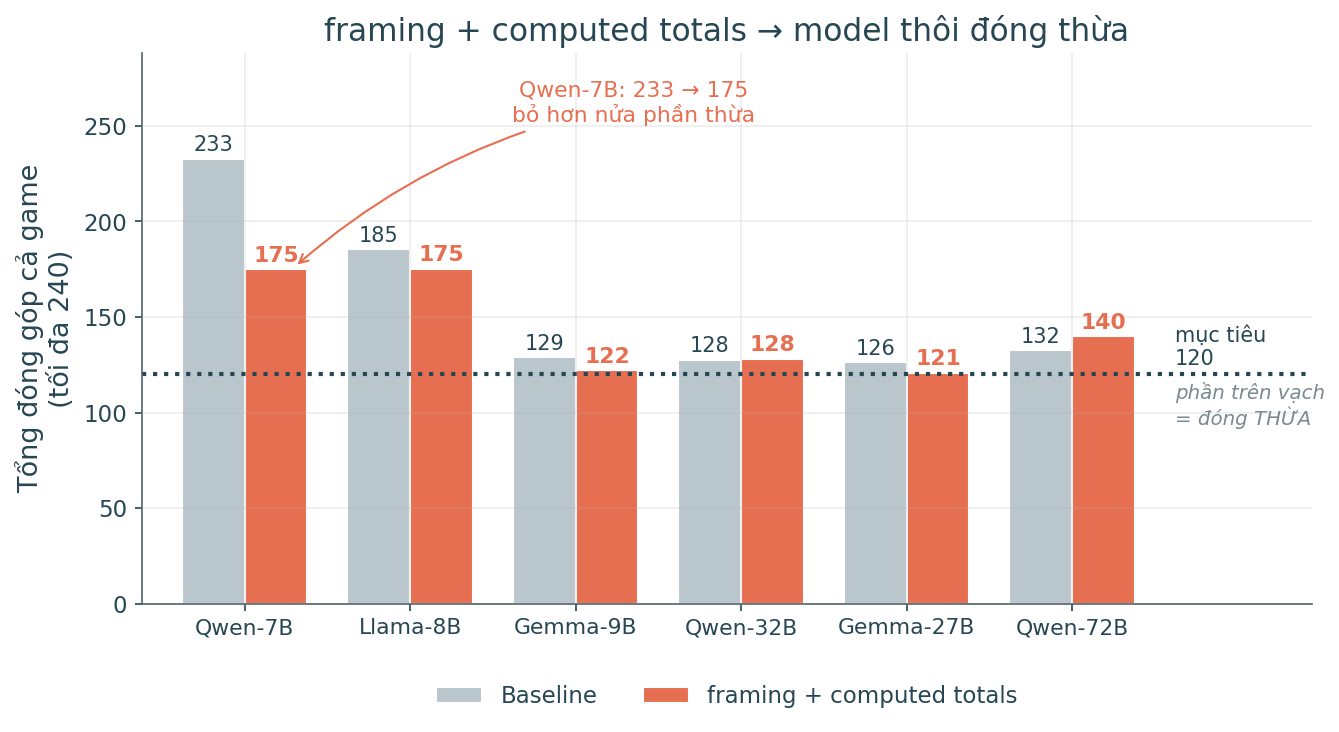
\includegraphics[height=0.66\textheight]{R1_excess.png}
  \take{Mục tiêu chỉ cần 120: Qwen-7B từ \weak{233} xuống \good{175}, Llama-8B \weak{185}$\to$\good{175},
  Gemma-27B về sát vạch \good{121}. Ba model vốn đã tiết kiệm thì gần như đứng yên.}
\end{frame}

\begin{frame}{Cơ chế: thấy ``đủ rồi'' là dừng ngay lập tức}
  \centering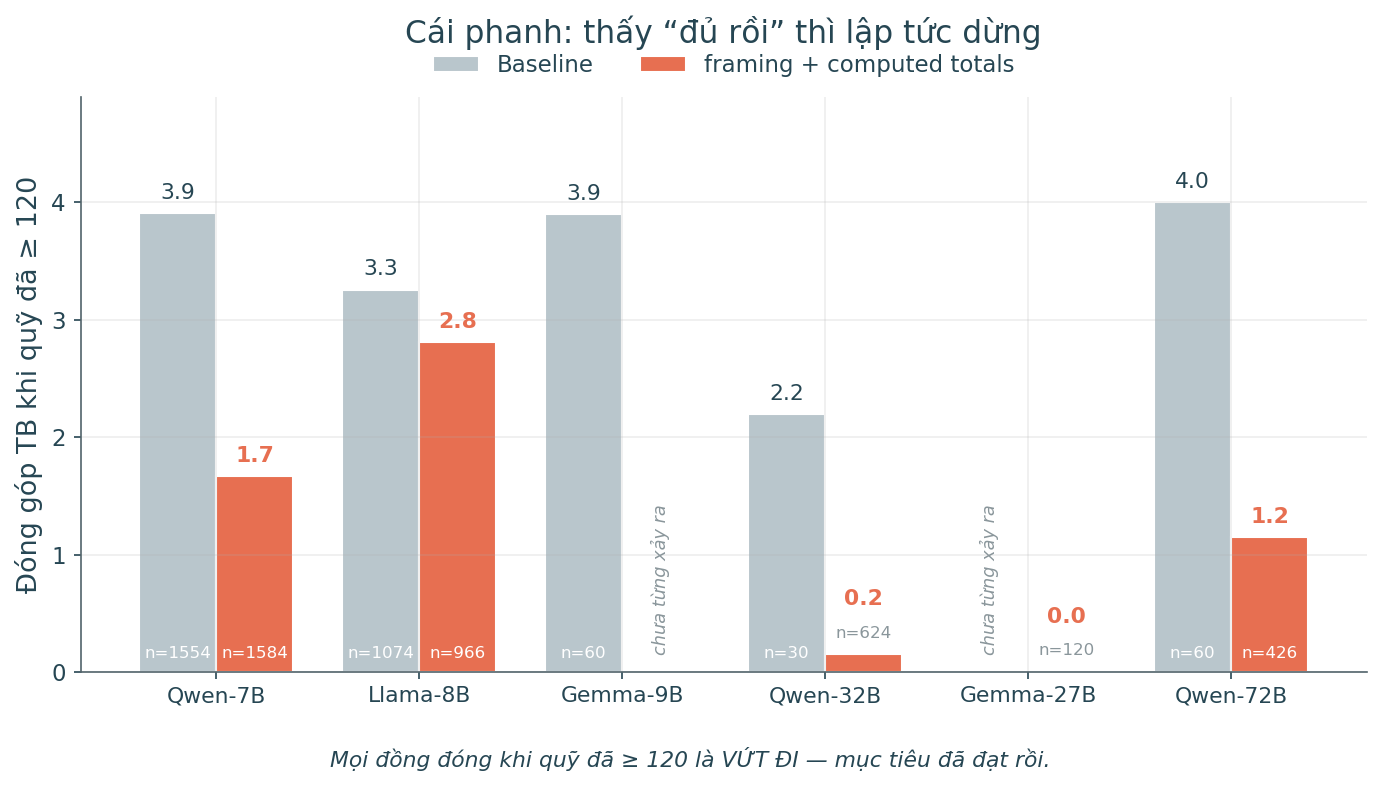
\includegraphics[height=0.64\textheight]{R3_brake.png}
  \take{Khi quỹ đã vượt 120, baseline vẫn đóng \weak{2--4 mỗi lượt} (tiền vứt đi).
  Nhánh \texttt{framing + computed totals}: Qwen-32B \good{0.2}, Gemma-27B \good{0.0}.}
\end{frame}

\begin{frame}{Nhịp chơi đổi hẳn: hết ``tăng dần tới chót''}
  \centering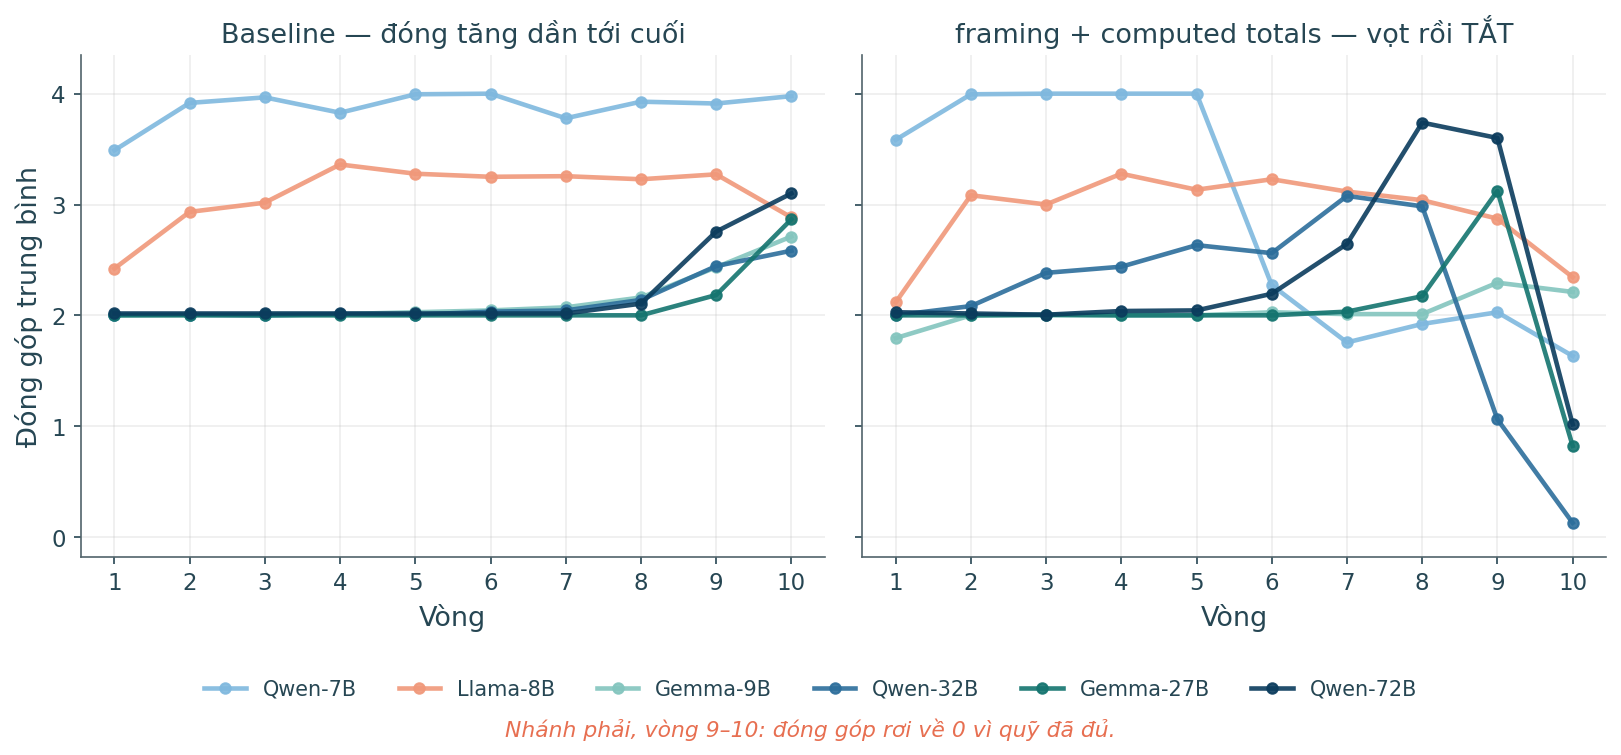
\includegraphics[height=0.60\textheight]{R4_dynamics.png}
  \take{Baseline: đóng tăng dần đến vòng 10 (ngược với người). Nhánh \texttt{framing + computed totals}:
  vọt lên khi còn thiếu rồi \good{tắt hẳn} khi đã đủ --- lần đầu thấy hình dạng ``đủ thì thôi''.}
\end{frame}

\begin{frame}{Vân tay lựa chọn: mức ``0'' lần đầu xuất hiện thật sự}
  \centering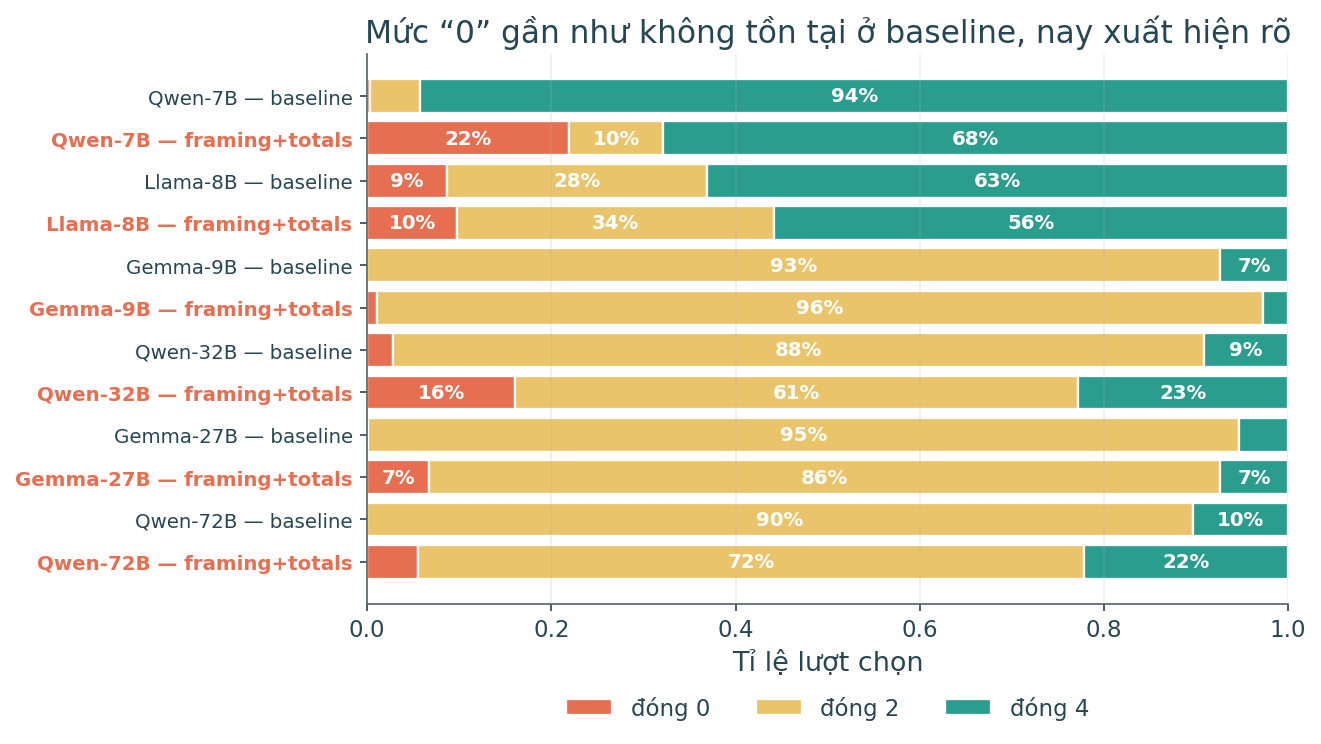
\includegraphics[height=0.72\textheight]{R8_choice.png}
  \take{Qwen-7B: \weak{0\%}$\to$\good{22\%} chọn 0; Qwen-32B \weak{3\%}$\to$\good{16\%}. Model học được cách \emph{không} đóng.}
\end{frame}

% ======================================================================
\section{Kết quả 2 --- cái KHÔNG được: vẫn không sợ rủi ro}

\begin{frame}{Phép thử cốt lõi vẫn trượt y như cũ}
  \centering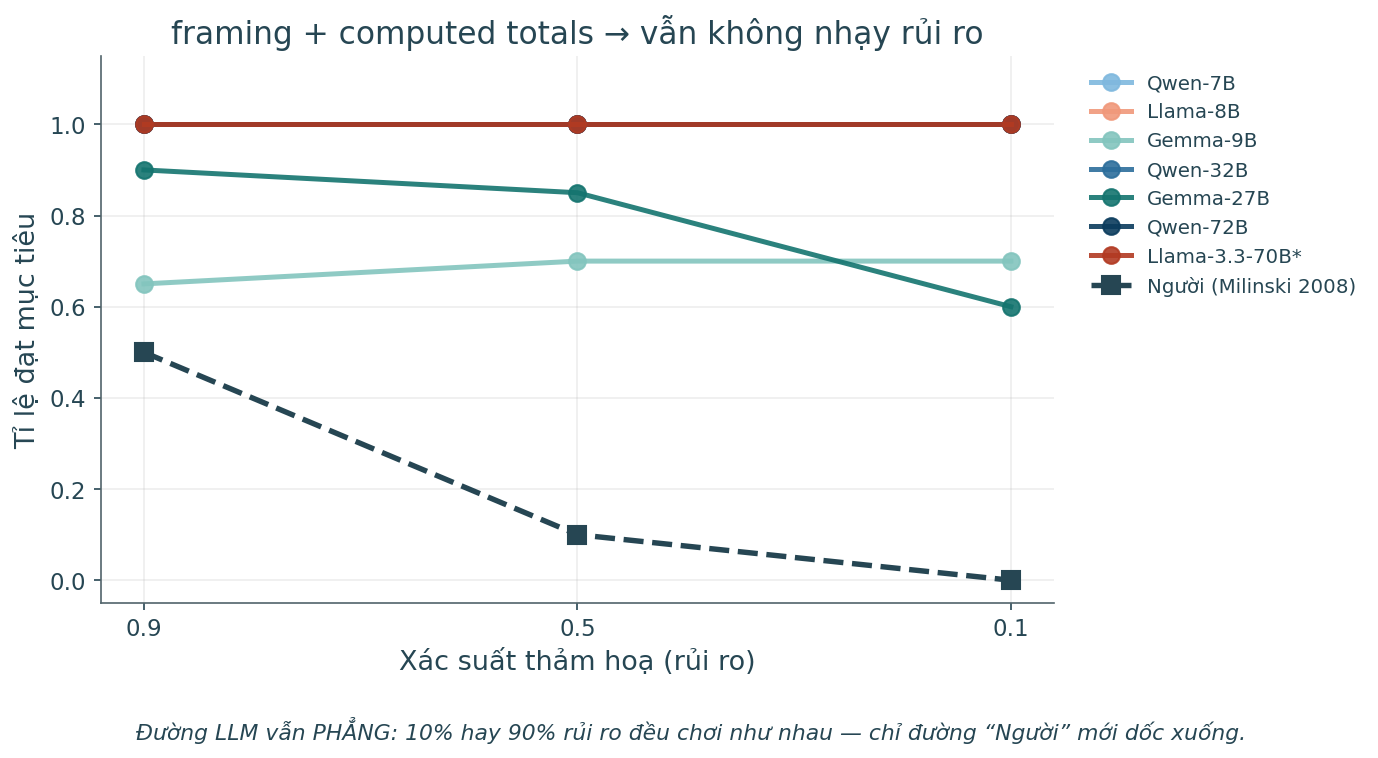
\includegraphics[height=0.66\textheight]{R2_reach_risk.png}
  \take{Nêu thẳng xác suất \emph{và} cho không con số $\Rightarrow$ đường vẫn \weak{phẳng}.
  Người đi từ 50\% xuống 0\%; LLM 10\% hay 90\% chơi hệt nhau.}
\end{frame}

\begin{frame}{Giả thuyết ``không tính nổi nên mới vậy'' bị loại}
  \begin{block}{Chuỗi loại trừ đã đi qua ba turn}
    \begin{itemize}\setlength\itemsep{3pt}
      \item Do model nhỏ? \;$\to$\; \weak{Không} (Turn 2: tới 72B vẫn phẳng)
      \item Do model mở / tự host? \;$\to$\; \weak{Không} (Turn 2: Gemini đóng y hệt)
      \item Do hiểu sai luật hay không biết mức rủi ro? \;$\to$\; \weak{Không} (Turn 2: $\sim$100\% đúng)
      \item Do phải tự cộng trạng thái nên không theo dõi được? \;$\to$\; \weak{Không} \alert{(Turn này)}
    \end{itemize}
  \end{block}
  \take{Cho không con số thì model \emph{dùng} ngay --- nhưng chỉ để tiêu ít đi, \good{không} để phản ứng với rủi ro.}
\end{frame}

% ======================================================================
\section{Kết quả 3 --- cái mất: chơi sát vạch rồi trượt}

\begin{frame}{Cái giá phải trả: Gemma từ 100\% xuống trượt vạch}
  \centering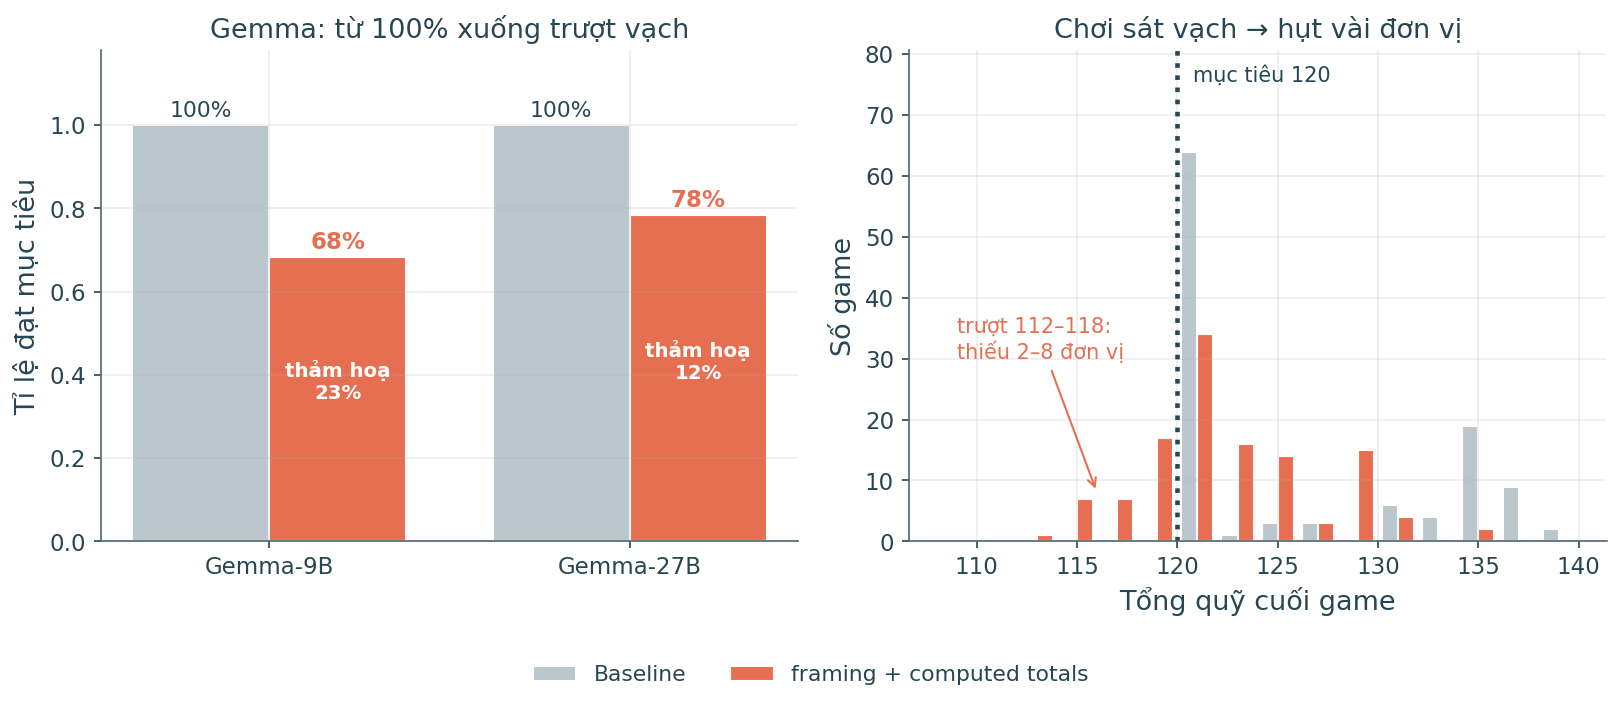
\includegraphics[height=0.60\textheight]{R5_gemma_cost.png}
  \take{Gemma-9B \weak{100\%$\to$68\%}, Gemma-27B \weak{100\%$\to$78\%}; thảm hoạ \weak{23\%} và \weak{12\%}.
  32 ván trượt đều rơi vào 112--118 --- \emph{hụt 2--8 đơn vị}.}
\end{frame}

\begin{frame}{Vì sao trượt? Con số dùng để DỪNG được, để BÙ thì không}
  \centering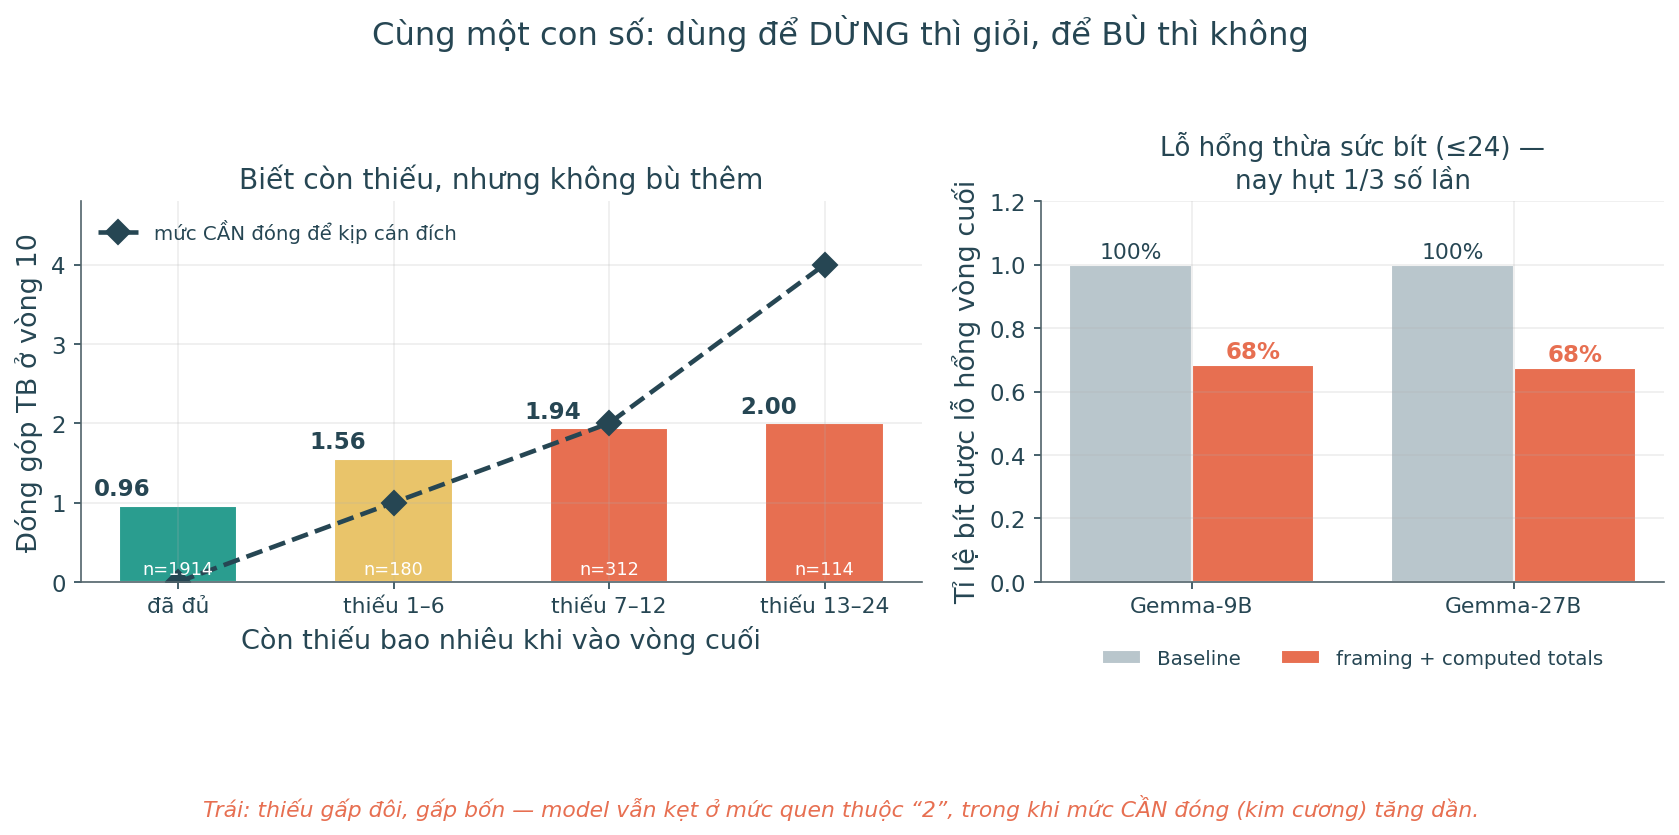
\includegraphics[height=0.58\textheight]{R6_asymmetry.png}
  \take{Thiếu 1--6 hay thiếu 13--24, model vẫn đóng $\approx$\weak{2} --- đúng mức quen thuộc.
  Ở Gemma, lỗ hổng vòng cuối thừa sức bít ($\le$24) nay \weak{hụt 1/3 số lần}.}
\end{frame}

\begin{frame}[fragile]{Ca tệ nhất: thiếu 2 đơn vị, rủi ro 90\%, cả nhóm đóng 0}
  \promptbox{\fontsize{6.8}{7.8}\selectfont}{assets/gemma_lastround.txt}
  \take{Model đọc đúng \good{118/120} và đúng \good{90\%}, rồi kết luận \weak{ngược}: ``đóng thêm bất kỳ số nào
  cũng có nguy cơ cao mất trắng''. Đóng 2 chính là thứ \emph{chặn} mất trắng.}
\end{frame}

\begin{frame}{Không phải lỗi số học --- là lỗi nối số vào hành động}
  \begin{block}{Ba mảnh khớp nhau}
    \begin{itemize}\setlength\itemsep{3pt}
      \item Model \good{đọc đúng} tổng quỹ (in sẵn) và \good{đọc đúng} mức rủi ro (Turn 2)
      \item Model \good{dùng được} con số cho một việc: \emph{đủ rồi thì dừng}
      \item Model \weak{không dùng} chính con số đó cho việc ngược lại: \emph{thiếu thì bù}
    \end{itemize}
  \end{block}
  \begin{exampleblock}{Nói gọn}
    Cho biết tổng quỹ là trao cho model một cái \good{phanh} --- không phải một cái \weak{vô lăng}.
  \end{exampleblock}
  \take{Trước Turn này ta ngờ lỗ hổng nằm ở \emph{số học}. Hoá ra số học chỉ là lớp ngoài.}
\end{frame}

% ======================================================================
\section{Ai được, ai mất}

\begin{frame}{Cùng một can thiệp, hai chiều tác động ngược nhau}
  \centering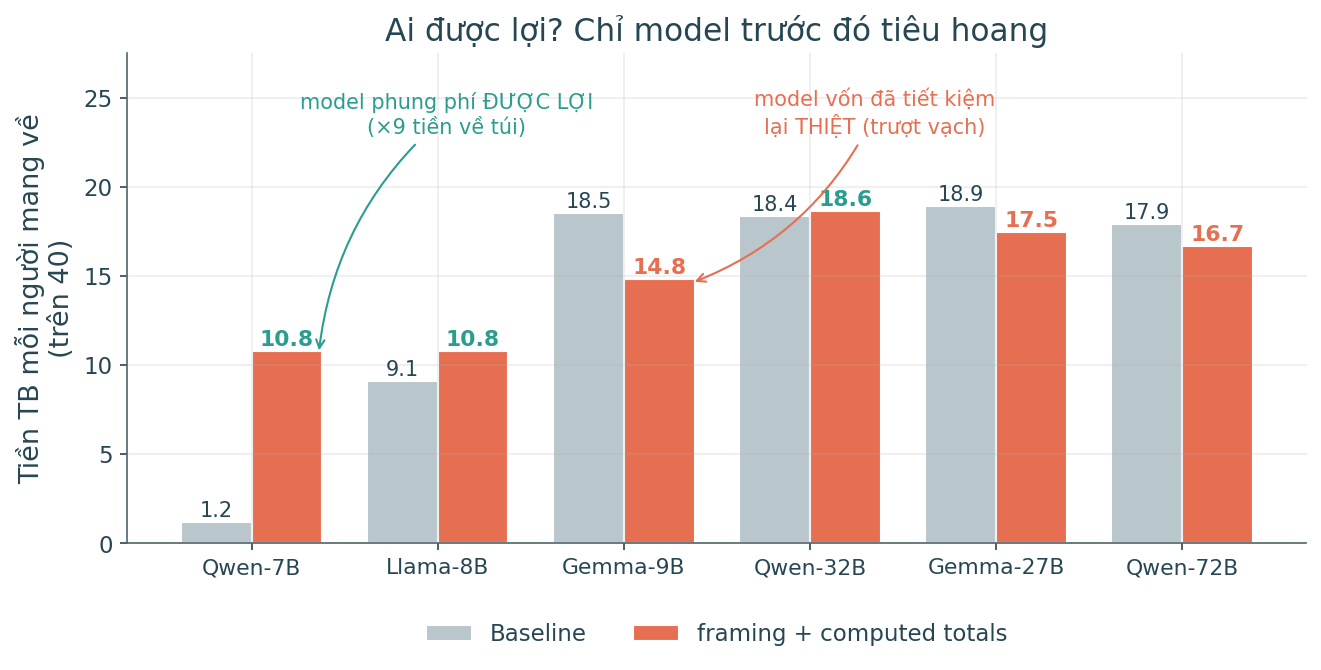
\includegraphics[height=0.62\textheight]{R7_payoff.png}
  \take{Model từng tiêu hoang \good{được lợi lớn} (Qwen-7B \weak{1.2}$\to$\good{10.8}, gấp 9 lần).
  Model vốn đã tiết kiệm thì \weak{thiệt} --- Gemma-9B 18.5$\to$\weak{14.8} vì mất luôn phần đệm an toàn.}
\end{frame}

\begin{frame}{Trục ngôn ngữ vẫn còn}
  \centering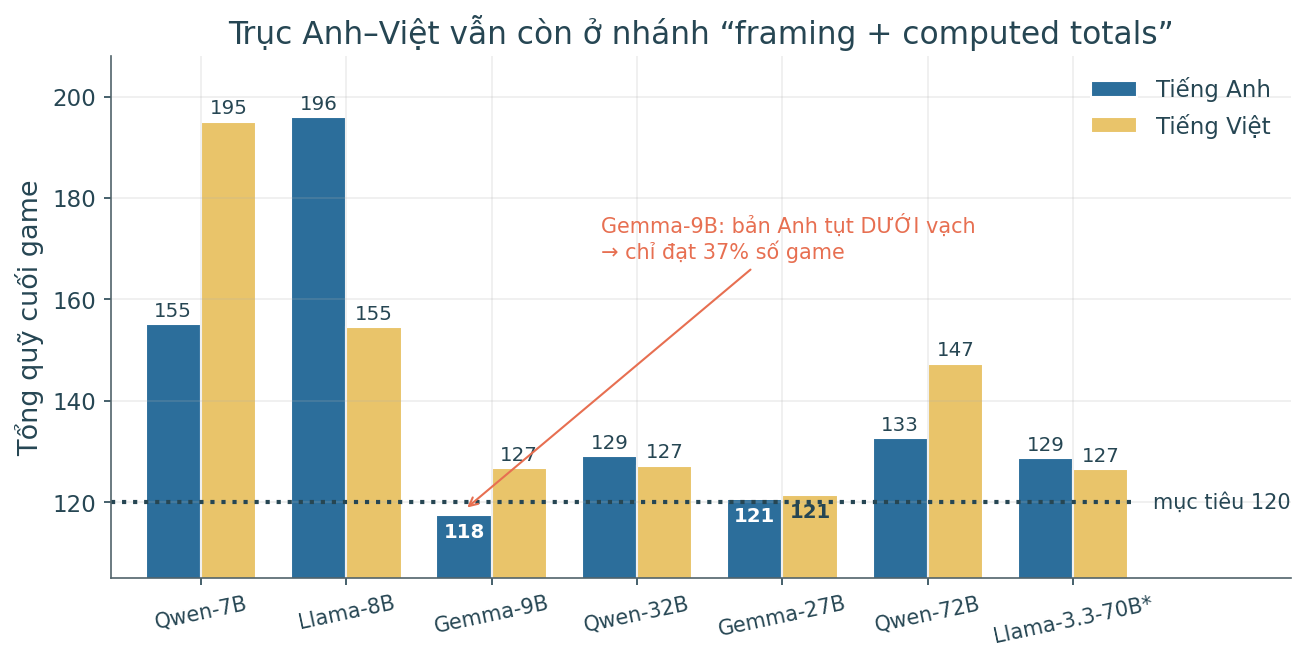
\includegraphics[height=0.60\textheight]{R9_lang.png}
  \take{Gemma-9B bản Anh tụt \weak{dưới vạch} (117.5) $\to$ chỉ đạt \weak{37\%} số ván, trong khi bản Việt
  \good{100\%}. Chênh lệch EN--VN không mất đi ở nhánh mới.}
\end{frame}

\begin{frame}{Bảng tổng hợp --- trước / sau}
  \centering
  \setlength{\tabcolsep}{6pt}\renewcommand{\arraystretch}{1.25}
  \begin{tabular}{lccc}
    \toprule
    & \textbf{Baseline} & \texttt{\textbf{framing + comp. totals}} & \\
    \midrule
    Tổng đóng góp (Qwen-7B)   & \weak{233} & \good{175} & tiết kiệm \\
    Tổng đóng góp (Gemma-27B) & 126        & \good{121} & sát vạch \\
    \rowcolor{hirow} Đóng góp khi quỹ đã đủ 120 & \weak{2--4} & \good{0.0--1.7} & \textbf{phanh ăn} \\
    Tiền mang về (Qwen-7B)        & \weak{1.2} & \good{10.8} & $\times 9$ \\
    \midrule
    \rowcolor{hirow} Phản ứng với rủi ro & Không & \weak{Vẫn không} & \textbf{không đổi} \\
    Tỉ lệ đạt (Gemma-9B / 27B)    & 100\% / 100\% & \weak{68\% / 78\%} & xấu đi \\
    Thảm hoạ (Gemma-9B / 27B)     & 0\% / 0\%     & \weak{23\% / 12\%} & xấu đi \\
    Bù lỗ hổng cuối, Gemma ($\le$24)& 100\%       & \weak{68\%}        & xấu đi \\
    \bottomrule
  \end{tabular}
  \take{Ba model còn lại (Qwen-32/72B, Llama-8B) giữ nguyên 100\% đạt mục tiêu --- chỉ tiêu ít đi.}
\end{frame}

% ======================================================================
\section{Tổng kết Turn 3}

\begin{frame}{Bức tranh sau ba turn}
  \begin{block}{Hợp tác của LLM là \emph{thói quen}, không phải \emph{tính toán} --- nay có bằng chứng trực tiếp}
    \begin{itemize}\setlength\itemsep{3pt}
      \item Cho không con số $\Rightarrow$ model \good{dùng ngay} để bỏ phần đóng thừa (Qwen-7B tiết kiệm hơn nửa)
      \item Cùng con số đó \weak{không} tạo ra phản ứng với rủi ro --- 10\% hay 90\% vẫn chơi như nhau
      \item Và \weak{không} tạo ra hành vi bù đắp: thiếu 2 hay thiếu 18, model vẫn đóng mức quen thuộc ``2''
      \item Gemma đọc đúng \emph{118/120} và \emph{90\%} mà vẫn kết luận ngược $\Rightarrow$ lỗi ở khâu
            \alert{nối con số vào quyết định}, không phải ở khâu đọc hay khâu cộng
    \end{itemize}
  \end{block}
  \take{Thông tin tốt hơn làm model \good{tiết kiệm hơn}, không làm nó \weak{an toàn hơn}.}
\end{frame}

\begin{frame}{So với hai turn trước}
  \centering
  \setlength{\tabcolsep}{9pt}\renewcommand{\arraystretch}{1.3}
  \begin{tabular}{lll}
    \toprule
    Câu hỏi & Turn 2 & Turn 3 \\
    \midrule
    Do model nhỏ / model mở?     & \weak{Không} & --- \\
    Hiểu luật, biết rủi ro?      & \good{Có}    & --- \\
    Do phải tự cộng trạng thái?  & giả thuyết   & \weak{Không} --- cho sẵn vẫn phẳng \\
    \rowcolor{hirow} Nhắc bài thì đổi gì? & chưa đo & \makecell[l]{\good{Hết đóng thừa} (phanh),\\\weak{không} hết phớt lờ rủi ro} \\
    Vì sao vẫn trượt?            & ``cộng dồn yếu'' & \makecell[l]{\weak{Không bù lỗ hổng} dù\\thấy rõ còn thiếu bao nhiêu} \\
    Trục ngôn ngữ?               & gây thất bại thật & \alert{Vẫn còn} (Gemma-9B EN 37\%) \\
    \bottomrule
  \end{tabular}
  \take{Turn này \emph{đóng} giả thuyết cuối cùng còn lại về nguyên nhân ``kỹ thuật''.}
\end{frame}

\begin{frame}{Điểm thảo luận với thầy}
  \textbf{Về thiết kế thí nghiệm}
  \begin{itemize}\setlength\itemsep{2pt}
    \item Turn này gộp hai thao tác vào một ô. Có cần chạy \alert{2$\times$2 đầy đủ} để tách riêng
          \texttt{framing} và \texttt{computed totals} không? (thêm 2 ô $\times$ 7 model $=$ 840 ván)
    \item Llama-70B ở arm này là bản \textbf{3.3}, baseline Turn 1 là bản \textbf{3.1} $\Rightarrow$ chưa so cặp
          sạch được; chạy lại 3.1 để khép bảng?
  \end{itemize}
  \smallskip
  \textbf{Về hướng đi tiếp}
  \begin{itemize}\setlength\itemsep{2pt}
    \item Bước tự nhiên kế tiếp: in sẵn luôn \alert{``còn thiếu bao nhiêu''} và \alert{``cần đóng bao nhiêu mỗi
          người''} --- nếu vẫn không bù thì loại nốt giả thuyết ``không suy ra được lỗ hổng''.
    \item Gemma trượt vì mất phần đệm an toàn: nên coi \emph{đệm dư} là hành vi phòng vệ hợp lý,
          hay là lãng phí? Ảnh hưởng cách diễn giải toàn bộ kết quả.
    \item Đưa arm frontier (gpt-nano / DeepSeek / Claude) vào cùng điều kiện này?
  \end{itemize}
\end{frame}

\begin{frame}[standout]
  Cho model \textbf{biết} tổng quỹ, nó lập tức \textbf{thôi đóng thừa}. \\[3mm]
  Cùng con số đó \textbf{không} làm nó sợ rủi ro hơn, \\
  và \textbf{không} làm nó bù vào chỗ còn thiếu. \\[3mm]
  {\normalsize Đó là một cái \textbf{phanh} --- không phải một cái \textbf{vô lăng}.}
\end{frame}

\end{document}
